\documentclass[a4paper]{article}

% Based on template: http://www.maths.lth.se/matematiklth/exjobb/exjobbarresurs/index.html

\usepackage[smartEllipses]{markdown}  % For markdown
\def\markdownOptionOutputDir{build}  % Needed, see https://github.com/Witiko/markdown/issues/6#issuecomment-328699108

\usepackage[dvipsnames]{xcolor}
\usepackage{hyperref}
\usepackage{comment}
\usepackage{xargs}
\usepackage{verbatim}
\usepackage{subfig}
\usepackage[bottom]{footmisc}
\usepackage[colorinlistoftodos, prependcaption, textsize=tiny]{todonotes}

% Add subsubsubsection
% As per https://tex.stackexchange.com/a/60212/36302
\usepackage{titlesec}
\setcounter{secnumdepth}{4}
\titleformat{\paragraph}
{\normalfont\normalsize\bfseries}{\theparagraph}{1em}{}
\titlespacing*{\paragraph}
{0pt}{3.25ex plus 1ex minus .2ex}{1.5ex plus .2ex}

% Code snippets
\usepackage[outputdir=build]{minted}
\usemintedstyle{vs}

\usepackage[english]{datetime2}
\DTMnewdatestyle{dashdate}{%
  \renewcommand{\DTMdisplaydate}[4]{\number##1-\DTMenglishshortmonthname{##2}-\number##3}%
  \renewcommand{\DTMDisplaydate}{\DTMdisplaydate}%
}
\DTMsetdatestyle{iso}

% From: https://tex.stackexchange.com/a/178806/36302
\newcommandx{\add}[2][1=]{\todo[linecolor=red, backgroundcolor=red!25, bordercolor=red, inline, #1]{\textbf{Add:} #2}}
\newcommandx{\unsure}[2][1=]{\todo[linecolor=red, backgroundcolor=red!25, bordercolor=red, #1]{\textbf{Unsure:} #2}}
\newcommandx{\change}[2][1=]{\todo[linecolor=blue, backgroundcolor=blue!25, bordercolor=blue, #1]{\textbf{Change:} #2}}
\newcommandx{\info}[2][1=]{\todo[linecolor=OliveGreen, backgroundcolor=OliveGreen!25, bordercolor=OliveGreen, #1]{\textbf{Info:} #2}}
\newcommandx{\improvement}[2][1=]{\todo[linecolor=Plum, backgroundcolor=Plum!25,bordercolor=Plum, #1]{\textbf{Improve:} #2}}
\newcommandx{\thiswillnotshow}[2][1=]{\todo[disable, #1]{#2}}

% Formatting
\setlength{\parindent}{0pt}
\setlength{\parskip}{1em}

% Encoding and languages
\usepackage[T1]{fontenc}        % För svenska bokstäver
%\usepackage[swedish]{babel}    %Svenska skrivregler och rubriker

% Graphics
\usepackage{epsfig}
%\usepackage[dvips]{graphics}

\newcommandx{\orcid}[1]{\href{https://orcid.org/#1}{
\includegraphics[width=0.7em]{img/orcid-icon.png}}}

\newcommand\myshade{85}
\colorlet{mylinkcolor}{violet}
\colorlet{mycitecolor}{YellowOrange}
\colorlet{myurlcolor}{Aquamarine}

\hypersetup{%
  linkcolor  = black, %mylinkcolor!\myshade!black,
  citecolor  = mycitecolor!\myshade!black,
  urlcolor = myurlcolor!\myshade!black,
  colorlinks = true,
}

% References
\usepackage[backend=biber, style=numeric, sorting=none, defernumbers=true]{biblatex}
\usepackage{cleveref}
\bibliography{zotero}
\bibliography{misc}
\DeclareBibliographyCategory{cited}
\AtEveryCitekey{\addtocategory{cited}{\thefield{entrykey}}}

\defbibheading{notcited}{\section*{Further Reading}}

\title{%
    \small DRAFT \today \\
    \small The latest version is available at \href{https://erik.bjareholt.com/thesis/thesis.pdf}{erik.bjareholt.com/thesis/thesis.pdf}\\
    \large --- \\
    \large \par M.Sc. Thesis\\
    \huge Classifying brain activity using low-cost biosensors and automated time tracking \\
}
\author{Erik Bjäreholt \orcid{0000-0003-1350-9677} \\(erik@bjareho.lt, dat13ebj@student.lu.se)}
\date{\today}

\begin{document}
\maketitle

\begin{abstract}

    We investigate the ability of EEG to distinguish between different activities users engage in on their devices, building on previous research which showed a considerable difference in brain activity when reading/(reasoning about) code vs prose.

    We also use the automated time tracker ActivityWatch, previously developed by the author, to track what activities the user is engaging in on their device while wearing an EEG device.

    \improvement[inline]{improve abstract}
\end{abstract}

\pagebreak %.\pagebreak

\tableofcontents

\listoftodos[Notes \& TODOs]

\pagebreak %.\pagebreak

\begin{refsection}

\section{Introduction}

    \add[inline]{Write introduction}

\section{Background}

    People spend more time than ever using computing devices. Work, entertainment, and services, have been steadily moving online over the last few decades and this trend is expected to continue.
    While several studies have been tracking how people spend time on their devices a wider study of how people's app usage is changing over time and how it varies with demographics, is not publicly available.

    Furthermore, how different device activities affect the user behaviorally and neurologically is of interest for many areas of research, including:

    \begin{itemize}
        \item psychological well-being, such as depression and social anxiety~\cite{selfhout_different_2009}\cite{shah_nonrecursive_2002}, stress~\cite{mark_stress_2014}, self-esteem, life satisfaction, loneliness, and depression~\cite{huang_time_2017}.
        \item the impact of screen time on children and adolescents~\cite{subrahmanyam_impact_2001}.
        \item attention span among media multitasking adults~\cite{mark_stress_2014}.
        \item enhancing personal productivity~\cite{kim_timeaware_2016}.
    \end{itemize}

    Understanding device use and the underlying cognitive processes are essential when designing for motivation, engagement and wellbeing in digital experiences~\cite{peters_designing_2018}.

    This becomes especially relevant for knowledge workers, such as software developers, who spend the majority of their working time on computing devices.

    \add[inline]{Mention of Quantified Self movement, and the applicability/usefulness of EEG data to the cause}

    %\add[inline]{Add connection to software developers}

\subsection{Automated time trackers}

    Automated time-trackers have been developed for computing devices, with various applications such as tracking hours worked, personal productivity, managing excessive use of social networking sites (SNSs), and studying human behavior.

    \subsubsection{Commercial use}

        Companies like RescueTime~\cite{noauthor_rescuetime_nodate}, Hubstaff~\cite{noauthor_hubstaff_nodate}, and others offer automated time tracking as a service. These services let the user track their screen time by installing a program on their device which tracks the active application and sends the data to their servers for storage and analysis. The user can then view their data in a dashboard on the service's website. Some of these services, like RescueTime and Hubstaff, are marketed towards teams and professionals, who want to keep track of individual and team productivity.

        However, these services have some issues for use by researchers and individuals alike. Notably, their collection of detailed and non-anonymized behavioral data into a centralized system bring significant privacy concerns, especially in cases where the data is shared with a team or an employer.

        Other limitations of these services, such as low temporal resolution and limited event detail, cause additional issues for certain tasks that are timing-sensitive (such as ERPs), or preprocessing steps that can take advantage of high level of detail (like classifying activity).

    \subsubsection{Research use}

        Previous research has been published which used automated time trackers, such as TimeAware~\cite{kim_timeaware_2016} and ScreenLife~\cite{rooksby_personal_2016}. However, these previous contributions are --- like the commercial services --- not open source nor permissively licensed, and therefore not available for external research use nor further development.

    \subsubsection{ActivityWatch}

        The free and open source automated time tracker ActivityWatch~\cite{bjareholt_activitywatch_2020} addresses aforementioned issues with other software around source availability/licensing, privacy, temporal resolution, event detail, and cross-platform support.

        \todo[inline]{Update screenshot to v0.11}

        \begin{figure}[h]
        \centering
        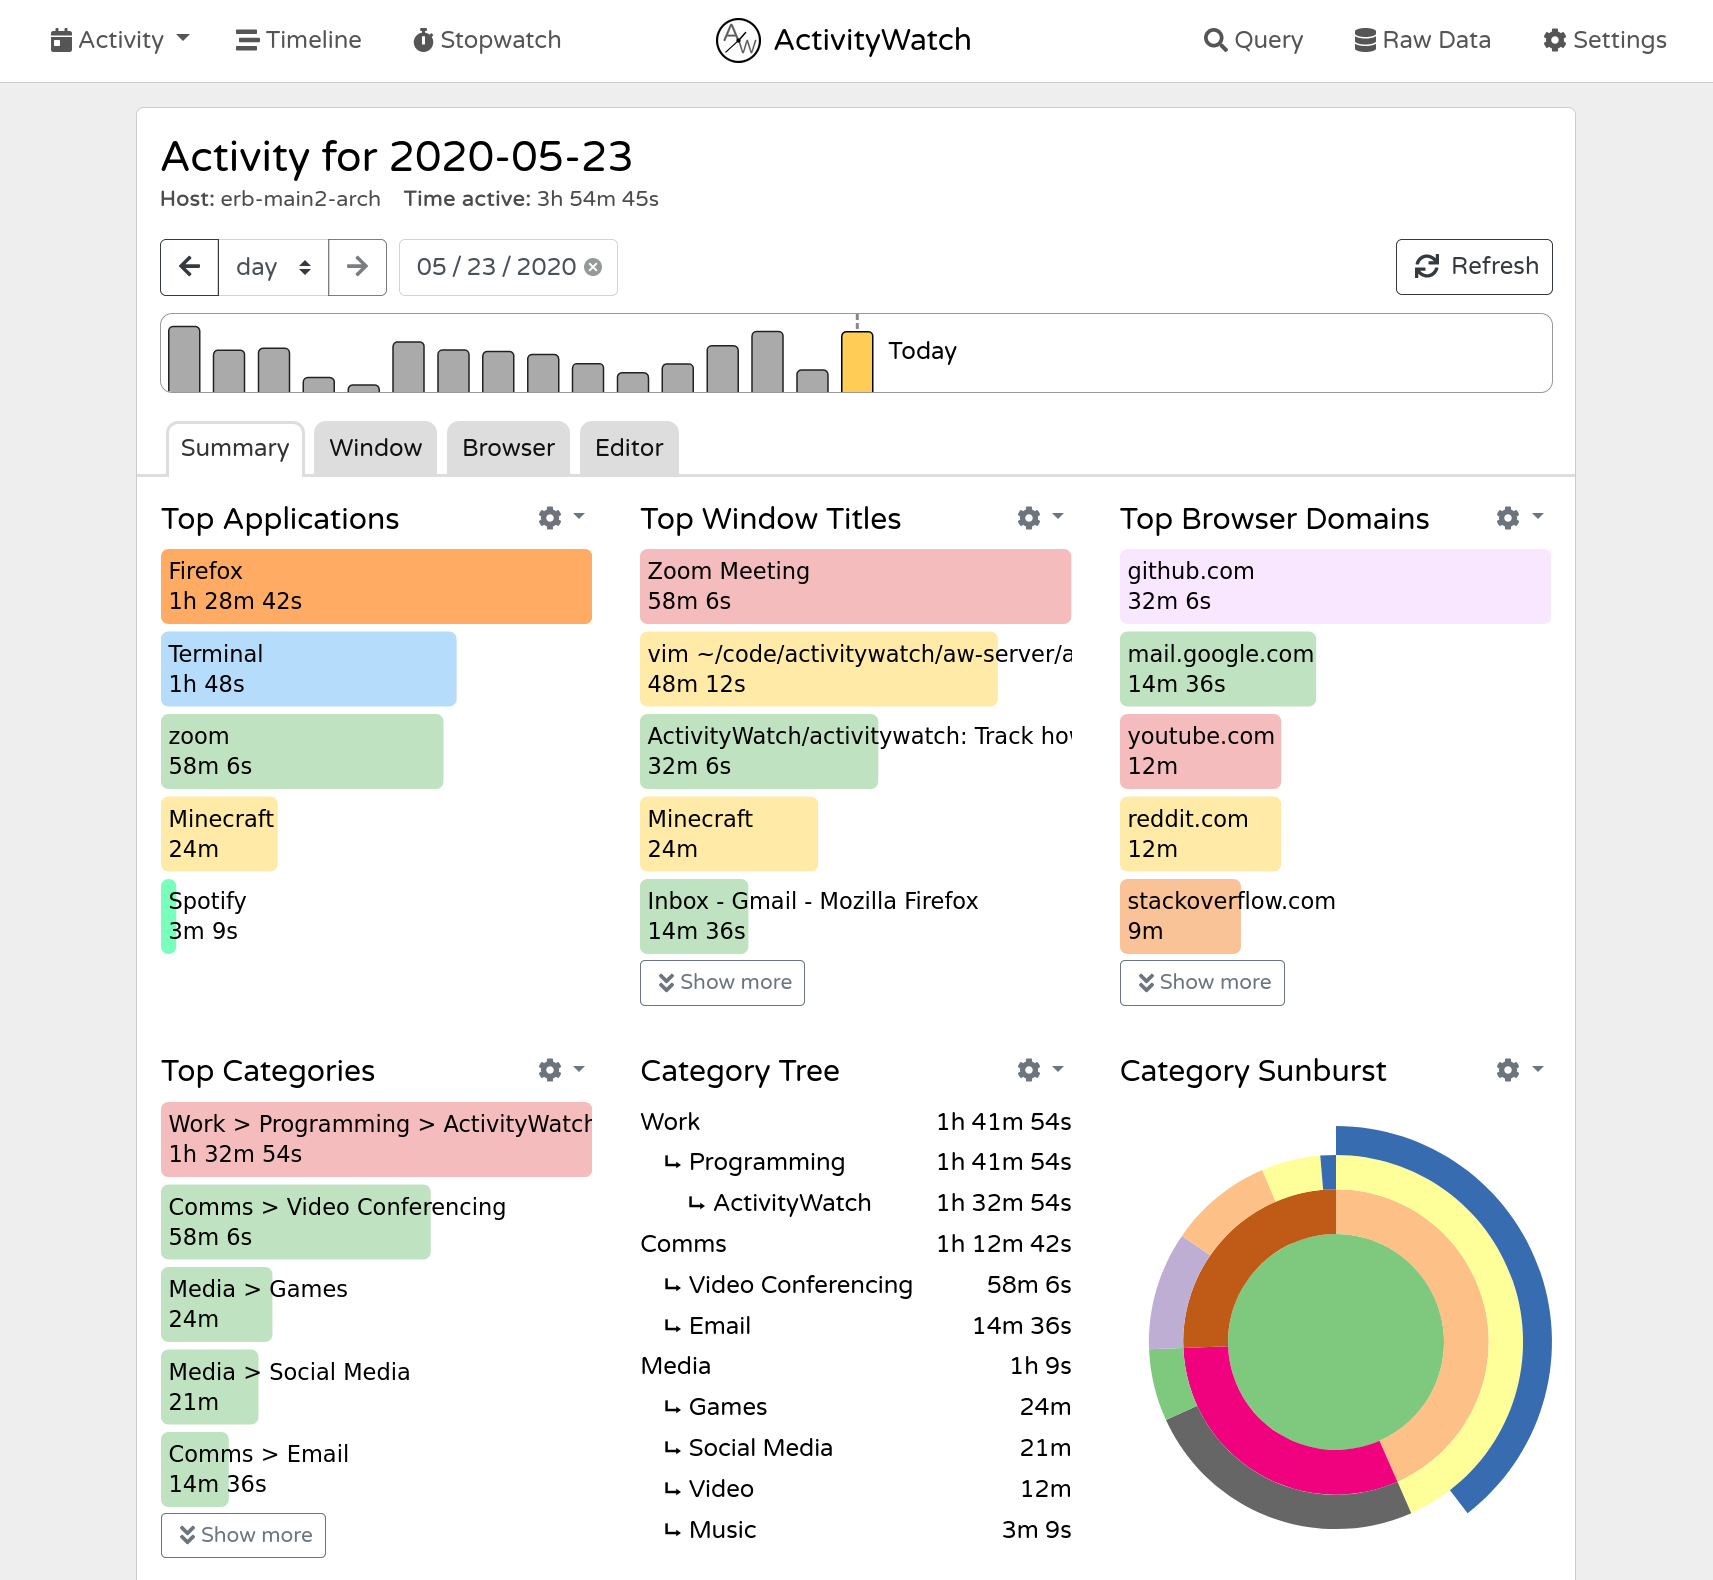
\includegraphics[width=12cm]{img/screenshot-aw-activity.png}
        \caption{ActivityWatch activity dashboard. Showing top applications, window titles, browser domains, and categories.}\label{fig:aw}
        \end{figure}

        ActivityWatch as a project was started in 2016 by the author of this thesis, with his brother Johan joining development soon after. It has since become a popular open source alternative to other time tracking software. It has received numerous contributions from users\footnote{Contributor statistics available at \href{https://activitywatch.net/contributors/}{activitywatch.net/contributors/}} and is approaching 100,000 downloads\footnote{Download statistics available at \href{https://activitywatch.net/stats/}{activitywatch.net/stats/}}.

        \todo[inline]{What more could I add about ActivityWatch? There should be relevant stuff in the docs, and in the slides I made way back.}

\subsection{EEG and low-cost biosensors/functional brain imaging}

    Functional brain imaging methods such as fMRI, fNIRS, and EEG, have been used to study the relationship between cognitive or physical activity, and brain activity~\cite{floyd_decoding_2017}\cite{hong_classification_2015}\cite{fucci_replication_2019}. The more accurate methods such as fMRI are costly and inflexible/impractical for many uses.

    However, the recent availability of low-cost biosensors such as EEG, HEG, and fNIRS, enables studying brain activity during real-life tasks. As an example it has been shown that it is possible to classify if a participant is reading code or prose using fMRI~\cite{floyd_decoding_2017}, which has been replicated using EEG and low-cost biosensors~\cite{fucci_replication_2019}. The ability to distinguish between these two tasks have been has been explained neurologically by the recruitment of different neural networks \todo[inline]{`neural network' might be confusing in the context} for the task. \todo[inline]{reference MIT paper}

    The code vs prose comprehension task has also been modified into a writing task studied under fMRI, to further shed light to the underlying brain activity. In one study it was found that code and prose writing are significantly dissimilar tasks for the brain, where prose writing engages brain regions associated with language in the left hemisphere while while code writing engages brain regions associated with attention, working memory, planning, and spatial cognition in the right hemisphere\cite{noauthor_neurological_nodate}.

    But they are not without their limitations --- among them a notably low signal-to-noise ratio~\cite{mcfarland_eeg-based_2017} --- yet visual evoked potentials (VEPs) have been shown to be sufficient for high-speed BCI applications~\cite{spuler_high-speed_2017}.

    To combat the low signal-to-noise ratio, machine learning methods have been employed with varying degrees of success. Examples from previous research include Convolutional Neural Networks (CNNs), which have been successful in classifying time series in general~\cite{zhao_convolutional_2017}, and EEG data in particular~\cite{schirrmeister_deep_2017}. As well as Hierarchical Convolutional Neural Networks (HCNNs), which have been used for EEG-based emotion recognition~\cite{li_hierarchical_2018}.

    \add[inline]{Applications to software engineers}

    \add[inline]{Separate sections for applications in BCIs vs neuroscience}

    % https://docs.openbci.com/citations

    % List of functional brain imaging techniques:
    %  - fMRI
    %  - fNIRS
    %  - EEG
    %  - HEG

\subsection{Aim of the thesis}

    The primary aim of the thesis is to improve upon previous attempts~\cite{fucci_replication_2019} to classify whether the user is reading code or prose using EEG data. This is to be achieved by using better EEG equipment and state of the art analysis methods such as Riemannian geometry. A secondary aim of the thesis is to investigate whether the ability of EEG analysis to classify code vs prose comprehension generalizes across more activities, such as the wide variety of tasks engaged in during organic device use.

    Secondary aims of the thesis include:

    \begin{enumerate}
        \item Implementing a classifier for device activities from EEG data, during organic device use
        \item Improving open-source tools for EEG analysis
    \end{enumerate}

    \add[inline]{Insert stuff from goal document}

\subsection{Related work}

    It has previously been shown that fMRI~\cite{floyd_decoding_2017} and EEG\cite{fucci_replication_2019} provides enough information to classify whether a subject is reading prose or code. However, accuracy with single-channel EEG has been found to be poor, and notably outperformed by a heart rate variability (HRV) monitor.

    % Here, we used functional magnetic resonance imaging to investigate two candidate brain systems: the multiple demand (MD) system, typically recruited during math, logic, problem solving, and executive tasks, and the language system, typically recruited during linguistic processing.
    Recently, it has been shown that the multiple demand (MD) system is typically recruited for code comprehension tasks, as opposed to the language system that is typically recruited during prose comprehension~\cite{ivanova_comprehension_2020}. This sheds light on the significant differences in how the brain processes code vs prose.

    In addition to purely studying comprehension (reading) code and prose, an 2020 fMRI study showed that there are indeed significant neurological differences between \emph{writing} code and prose as well.

    In software engineerig, low-cost biosensors such as wristbands that measure electrodermal activity and heart-related metrics have been used for emotional detection, as a tool in studying developer productivity.

    \add[inline]{Insert mention of preprint that Fucci mentioned?}

\section{Theory}

    \subsection{Electroencephalography (EEG)}

        Electroencephalography is a method used to measure the activity of neurons in the brain by recording the electrical activity on the scalp.

        As a non-invasive method it is widely used in medicine to diagnose and study a wide range of conditions, from epilepsy to sleep disorders.

        In research it has also found use in studying ``Event Related Potentials'', or ERPs, which are stereotypes responses to a stimulus. Common ERPs include N170, which 

        \add[inline]{Explain theory used, like theory of EEG, Riemannian geometry, etc}
        \add[inline]{Plots of raw EEG signal, PSD, PCA, etc}

        As measurements are taken on the scalp, neural activity of surface-level neurons can be expected to dominate the signal, which makes it difficult to use when studying systems deeper in the brain, such as the hippocampus. As an example of this, eye blinks are easily identifieable in the signal when electrodes are placed on the frontal cortex.

        \add[inline]{Plot of signal during eye blink}

    \subsection{Machine Learning}

        Machine learning on EEG data utilizes several domain-specific methods (which?) often similar to other methods seen applied to general time-series data.

        Among these we find methods like bandpass filtering, windowing, spectral density estimation, and the computation of covariance matrices to find interdependencies between channels.

        Common methods used in analysis and classification of EEG data include Linear Discriminant Analysis (LDA), Common Spatial Pattern (CSP) filters.

        With the use of these methods, we can compute features to use when training our classifiers.

        The underlying ML algorithms themselves are often off-the-shelf linear , with some domain adaptations found in more complex models like neural networks.

        \add[inline]{Formulas}

        \subsubsection{Riemannian geometry}

            \add[inline]{Explanation of Riemannian geometry, from \href{https://colab.research.google.com/drive/1y9tq7-lJwusxtVgpB38y-p1pYw7hg0iu}{this tutorial we're working on}, perhaps it should go in the Background/Theory section though?}

\section{Method}

    \subsection{Collection}

    \subsubsection{Collection of device activity data}

        All device activity is collected using the automated time tracker ActivityWatch~\cite{bjareholt_activitywatch_2020-1}.

        ActivityWatch collects data through modules called watchers which report to the ActivityWatch server. It comes with two watchers by default:

        \begin{itemize}
            \item aw-watcher-window, tracks the active window and its title
            \item aw-watcher-afk, tracks if the user is active or not by observing input device activity
        \end{itemize}

        A limitation that we have to consider is that the window watcher uses a polling method to track the active window, with a default poll time of 1 second. This means that we can't rely on the timestamps to mark the exact time the window became active/inactive.

        The data from ActivityWatch is processed and categorized such that the resulting data has the 3 columns \mintinline{python}{start, end, category}. The category is determined by a regular expression that matches on window titles and URLs, such as \mintinline{python}{github.com}.

    \subsubsection{Collection of EEG data}

        EEG data was collected during organic device use and under controlled conditions.

        For both conditions, code from the open source eeg-notebooks~\cite{noauthor_neurotechxeeg-notebooks_2020} was adapted to record the raw EEG stream into a CSV file. For the Muse S, muse-lsl~\cite{muse-lsl} was used as the underlying software to handle the connection (which uses Lab Streaming Layer). For the OpenBCI and Neurosity devices, brainflow~\cite{noauthor_brainflow-devbrainflow_2020} was used to handle the connection.

        \paragraph{During organic device use}

            For the organic device use conditions, we primarily used the Muse S EEG headband which features 4 channels with electrodes placed at TP9, AF7, AF8, and TP10.\footnote{According to the 1020-system.} The Muse S was chosen mainly due the superior comfort and ease of use compared with the alternatives, making it especially suitable for long recordings.\footnote{A wet electrode cap system was also considered, but ultimately not investigated due to being inconvenient to setup.}

        \paragraph{During code vs prose comprehension task}

            For the controlled condition, the hardware used was \todo[inline]{decide on which hardware to use}{\ldots}.

            We \todo{actually implement the task}{implemented the task} in eeg-notebooks~\cite{noauthor_neurotechxeeg-notebooks_2020}, which uses previously mentioned libraries for data collection as well as PsychoPy~\cite{peirce_psychopy2_2019} to provide the stimuli.

            \todo[inline]{actually perform controlled experiments}

        \paragraph{Devices}

            The Muse S is a 4-channel EEG headband with electrodes at TP9, AF7, AF8, and TP10, with the reference electrode at Fpz~\cite{krigolson_choosing_2017}.

            \todo[inline]{Add images of headsets}

            \begin{center}
                \begin{table}
                \begin{tabular}{llccc}
                    Manufacturer
                    & Device
                    & Channels
                    & Sampling rate
                    & Comfort
                    \\
                    InteraXon
                    & Muse S
                    & 4
                    & 250Hz
                    & High \\
                 OpenBCI
                    & Cyton (with Ultracortex)
                    & 8
                    & 125Hz?
                    & Low \\
                 % generously gifted by Neurosity
                 Neurosity
                    & Notion DK1
                    & 8
                    & 250Hz?
                    & Medium \\
                  % preordered, arrives in late spring
                  Neurosity
                    & Crown
                    & 8?
                    & 250Hz?
                    & High? \\
                \end{tabular}
                \caption{Devices used}
                \end{table}
            \end{center}

            \begin{center}
            \begin{figure}
                \begin{tabular}{cc}
                    img1 %\includegraphics[width=65mm]{it}
                    & img2 %\includegraphics[width=65mm]{it}
                    \\
                    (a) Muse S
                    & (b) OpenBCI Cyton with Ultracortex
                    \\[6pt]
                    img3 %\includegraphics[width=65mm]{it}
                    & img4 %\includegraphics[width=65mm]{it}
                    \\
                    (c) Notion DK1
                    & (d) Notion Crown
                    \\[6pt]
                \end{tabular}
                \caption{Photos of devices used}
            \end{figure}
            \end{center}

    \subsection{Analysis}

        For classification and analysis, we used common open source Python libraries for data analysis, like numpy~\cite{harris2020array}, pandas~\cite{reback2020pandas}, and scikit-learn~\cite{scikit-learn}. In addition, we used less common libraries tailored specifically for working with EEG data, such as MNE~\cite{noauthor_mne-toolsmne-python_2020}, pyriemann~\cite{alexandre_barachant_2020_3715511}, and YASA~\cite{raphael_vallat_raphaelvallatyasa_2020}.

        \subsubsection{Data cleaning}

            For the uncontrolled condition, we align the raw EEG data with the categories assigned by our ActivityWatch script. We split the series into epochs, and reject samples that either:

            \begin{enumerate}
                \item Don't have an assigned class
                \item Have a bad signal quality (as indicated by a high signal variance)
                \item Are too short (due to missing samples)
            \end{enumerate}

            \todo[inline]{List how many epochs are rejected by each cleaning step}

        \subsubsection{Feature engineering}

            \paragraph{Bandpower}

                Bandpower features are simple and commonly used in EEG research for many tasks, including the paper by Fucci et al we seek to improve upon~\cite{fucci_replication_2019}. As a reference, we implemented classifiers which solely used bandpower features as input, to gain information of how much any improvement from classifier performance is likely due to better EEG equipment versus how much is due to from improved analysis methods.

                To compute this feature, we utilized the bandpower function provided by YASA~\cite{raphael_vallat_raphaelvallatyasa_2020}. The implementation estimates the power spectral density using Welch's method for each channel, and bins them by their associated frequency band.

            \subsubsection{Riemannian geometry}

                The \improvement{according to whom?}{state of the art in many EEG classification tasks} involves the use of Riemannian geometry. For this, we used the open source pyriemann library by Alexandre Barachant\footnote{First author of the original paper to apply Riemannian geometry to EEG~\cite{barachant_classification_2013}}.

        \subsubsection{Neural Networks}

            One of the classifiers we want to train is a neural network. We use braindecode~\cite{schirrmeister_deep_2017}\cite{noauthor_braindecodebraindecode_2021}, a neural network toolbox for EEG data that uses PyTorch and integrates it with scikit-learn through skorch.

            The networks provided by braindecode are\ldots

        \subsubsection{Cross Validation}

            We use LORO (``Leave-One-Run-Out'') cross-validation, a variation of LOGO (``Leave-One-Group-Out''), in order to ensure the samples used in validation are using subjects or tasks that are unseen in training.

            We attempt both out-of-subject validation and out-of-task validation in order to estimate the ability of the classifiers to generalize across subjects and tasks.



\section{Results}

    \subsection{Code vs prose task}

        Our top-performing classifier yields a LORO-CV score of\ldots.

        Our classifier performance is\ldots

    \subsection{Naturalistic device activity}

        Our classifier performance is\ldots

\section{Conclusions}

    Our results show that it is possible to distinguish between reading code and prose, and improves upon the state of the art in this regard.

    Furthermore, our naturalistic experiments indicate it is possible to distinguish many other device activities from each other using consumer-grade EEG devices. Among these some data seems to suggest that EEG is sufficient to not only pick up differences in code vs prose \emph{comprehension} but also \emph{writing}.

\section{Discussion}

    \subsection{Ethical considerations}

        When studying EEG data a range of ethical considerations arise. 

        \begin{itemize}
            \item Could the data be considered personally identifiable information (PII)? 
            \item How privacy sensitive are EEG recordings? Could they contain something the subject would rather keep private? (could have medical implications)
        \end{itemize}

        Companies such as Neurosity have taken an approach with their products where all the processing happens on-device, and only aggregates and classifier outputs are sent to the cloud for storage and presentation to the user.

        \add[inline]{Discuss ethics/privacy considerations of data collection, how it's dealt with in ActivityWatch, and implications of results on similar concerns apply to EEG data}

        \add[inline]{Mention OpenMined, https://github.com/OpenMined/PySyft, and similar tech (esp in the context of crowdsourcing data)}

    \subsection{Democratization of neuroscience}

        \add[inline]{Write about democratization efforts, like eeg-notebooks, and how it fits into the larger picture of EEG equipment becoming cheap and widely available.}

        This thesis was made possible due to the efforts of individuals and communities such as NeuroTechX to democratize neuroscience. Indeed, it is the explicit goal of the NeuroTechX eeg-notebooks project to `democratize the neuroscience experiment'. Combined with the rapid cost reduction of research-grade EEG equipment over the last decade it has enabled any programmer to design and perform high-quality neuroscience experiments.

        \todo[inline]{Mention the research process of going from costly fMRI (to reveal mechanisms) to cheaper EEG/fNIRS/etc (to put the research into practice)}

        As development of BCIs advance and the consumer market for EEG devices grow (as evidenced by new devices being released with a regular cadence by InteraXon and Neurosity) we expect to see more uses and applications of these devices.

        Much of this work was made possible due to the efforts of communities such as NeuroTechX to democratize neuroscience by publishing tools and code for running experiments.

    \subsection{Crowdsourcing data}

        Collecting data is a significant time sink for researchers, and efforts to crowdsource data from the general public are difficult for EEG as it still requires access to the equipment, the knowledge to operate it, as well as considerations like signal quality, electrode placement, and other factors that might invalidate the data.

        As part of the thesis work I've contributed to an effort in crowdsourcing EEG data collected from the experiments built in eeg-notebooks using consumer EEG devices like the Muse and OpenBCI\@. The effort, called the \href{https://neurotech-challenge.com/}{NeuroTech Challenge Series} (NTCS), is lead by John Griffiths at the University of Toronto.

        \add[inline]{Write about crowdsourcing of EEG data, including the potential of transfer learning and privacy considerations.}

\section{Other contributions}

    As part of the work on this thesis I've contributed several improvements to the open source projects used, including muse-lsl, moabb, eeg-notebooks, and pyRiemann.

    \begin{itemize}
        \item \href{%
                https://github.com/search?q=org%3ANeuroTechX+is%3Apr+sort%3Aupdated-desc+author%3AErikBjare
            }{PRs to NeuroTechX repos (eeg-notebooks, moabb) (22)}
        \item \href{%
                https://github.com/search?q=org%3Aalexandrebarachant+is%3Apr+sort%3Aupdated-desc+author%3AErikBjare
            }{PRs to Alexandre Barachant repos (muse-lsl, pyRiemann) (4)}
        \item \href{%
                https://github.com/search?q=org%3Abraindecode+is%3Apr+sort%3Aupdated-desc+author%3AErikBjare
            }{PRs to the braindecode repo (1)}
    \end{itemize}

\section*{Acknowledgements}

\begin{itemize}
 \item My advisor Markus Borg~\orcid{0000-0001-7879-4371}.
 \item My brother Johan Bjäreholt, for working with me on ActivityWatch all these years.
 \item The NeuroTechX crowd, specifically Morgan Hough~\orcid{0000-0001-5256-413X} and John Griffiths, for their support and time spent helping me.
 \item The people at the LTH Department for Automatic Control, for providing early guidance.
 \item Andrew Jay Keller at Neurosity, for giving me a refurbished Notion DK1 to work with.
 \item Alex K. Chen, for referring me to all the right people.
 \item All the test subjects.
 \item Everyone who's contributed to the open source tools I've used.
\end{itemize}

    The Oxford English Dictionary defines `thesis' as ``a long essay or dissertation involving \emph{personal research}, written by a candidate for a university degree''. I can't think of more ``personal research'' than research in quantified self with personal data.


% References
%\bibbysegment{}
\printbibliography[category=cited]

% Further reading (uncited)
\nocite{*}
\defbibenvironment{bibnonum}
  {\list{}
     {\setlength{\leftmargin}{\bibhang}%
      \setlength{\itemindent}{-\leftmargin}%
      \setlength{\itemsep}{\bibitemsep}%
      \setlength{\parsep}{\bibparsep}}
  }
  {\endlist}
  {\item}
\printbibliography[notcategory=cited, env=bibnonum, heading=notcited]

\end{refsection}
\end{document}
